\chapter{Literatuuronderzoek}
\label{ch:literatuuronderzoek}

De eerste fase in elk onderzoek is typisch om een overzicht te schrijven van de huidige stand van zaken in het onderzoeksdomein. Daarvoor is het nodig om je te verdiepen in \emph{alles} wat er over het onderwerp al geschreven is. Dit is het literatuuronderzoek. In elk verslag over onderzoek is het essentieel dat je elke bewering die je doet ook kan aantonen. Dat kan ofwel op basis van data die je zelf op een methodologisch correcte manier verzameld en geanalyseerd hebt (maar dat komt verder in deze gids aan bod), ofwel aan de hand van refererenties naar \emph{gezaghebbende} publicaties.

Dit hoofdstuk gaat dieper in op dit onderwerp: wat bereik je precies met een literatuurstudie, hoe kan je er aan beginnen, hoe kan je de bronnen die je vindt gestructureerd bijhouden en op welke manier gebruik je die dan in je tekst?

HOGENT heeft via Chamilo een cursus over informatievaardigheden gepubliceerd\footnote{\url{https://chamilo.hogent.be/index.php?go=CourseViewer\&application=Chamilo\%5CApplication\%5CWeblcms\&course=22068\&tool=LearningPath\&browser=Table\&tool_action=ComplexDisplay\&publication=980981}} die je zeker eens moet doornemen. Het is immers niet de bedoeling om in deze gids dezelfde inhoud te herhalen. Dit hoofdstuk spitst zich in de eerste plaats toe op literatuuronderzoek over een ict-gerelateerd onderwerp, en het correct opmaken van een referentielijst met {\LaTeX} en JabRef (zie Sectie~\ref{sec:bibliografische-databank}).

Neem ook opnieuw de cursus Onderzoekstechnieken bij de hand, in het bijzonder het lesmateriaal ivm {\LaTeX} en rapporteren over onderzoek.

\section{Doel van het literatuuronderzoek}
\label{sec:doel-literatuuronderzoek}

Het belangrijkste doel van een literatuuronderzoek is om vertrouwd te worden met het onderzoeksdomein en die kennis ook door te geven aan de lezers van je bachelorproef. Je gaat dus zoveel mogelijk informatie verzamelen en lezen over het onderwerp zodat je er eigenlijk alles over weet dat er op dit moment over te weten valt. Het is dan de bedoeling om alle voor je onderzoek relevante kennis die je op deze manier hebt opgedaan ook op een gestructureerde manier en in je eigen woorden samen te vatten in een doorlopende tekst. Dit vormt meestal het eerste hoofdstuk (of de eerste hoofdstukken) van je bachelorproef.

Aan de hand van de literatuurstudie geef je de lezer de nodige achtergrond om het onderwerp te begrijpen. Het is een inleiding op het onderwerp, en bespreekt de huidige stand van zaken. Je vermeldt wat de experten in het domein er over te zeggen hebben en welk onderzoek er in het verleden al over gedaan is (met uiteraard vermelding van de belangrijkste conclusies). Uit de literatuurstudie moet ook naar voor komen dat er nog hiaten in onze kennis zijn, dat er een probleem is dat om een oplossing vraagt. En dat is uiteraard precies het onderwerp van je bachelorproef.

\section{Soorten bronnen}
\label{sec:soorten-bronnen}

In het kader van een onderzoek kunnen we informatiebronnen ondeverdelen in deze drie categorieën:

\begin{description}
  \item[Primaire] kennis die je zelf vergaart tijdens je onderzoek. Bijvoorbeeld metingen uit experimenten, resultaten van enquêtes, transcripties van interviews, enz.
  \item[Secundaire] publicatie van kennis, onderzoek, enz.~door anderen. Bijvoorbeeld artikels in vaktijdschriften, boek, presentatie op een conferentie, enz.
  \item[Tertiaire] zoekindexen en encyclopedieën. Bijvoorbeeld Google Scholar, Web of Science, Elsevier ScienceDirect, Arxiv.org, Wikipedia, about.com, Webopedia, enz.
\end{description}

Wanneer in een tekst verwezen wordt naar de literatuur, dan gaat het telkens over \emph{secundaire} bronnen (ook \emph{publicaties} genoemd). Dat betekent ook dat primaire of tertiaire bronnen \emph{niet} kunnen. Er mag dus bijvoorbeeld nooit verwezen worden naar een Wikipedia-artikel, woordenboeken, enz. Tertiaire bronnen zijn wel goede \textit{startpunten} van de zoektocht naar geschikte publicaties (Zie Sectie~\ref{sec:op_zoek_naar_relevante_informatie}). Je kan ook niet verwijzen naar het verslag van een interview dat je gevoerd hebt, omdat dat ook niet gepubliceerd is en dus niet toegankelijk voor de lezer.

\subsection{Publicatievormen}
\label{sub:publicatievormen}

Kennis wordt doorgegeven en gepubliceerd in verschillende vormen. In deze sectie lijsten we de belangrijkste op en bespreken de betrouwbaarheid en objectiviteit van elk.

\paragraph{Artikel in wetenschappelijk tijdschrift}

Van een artikel dat in een wetenschappelijk tijdschrift (of Eng. \emph{journal}) gepubliceerd wordt, mag je uitgaan dat er eerst een rigoreus verificatieproces aan vooraf gegaan is. Ingezonden artikels worden door de redacteurs van het tijdschrift doorgegeven aan andere experten in het vakgebied die de verantwoordelijkheid hebben de inhoud ervan op een onafhankelijke manier te verifiëren. Dit noemt men in het Engels \emph{peer review}. Dit proces duurt typisch verschillende maanden en kan zelfs uitlopen tot een paar jaar. Publicaties in wetenschappelijke tijdschriften worden algemeen beschouwd als de meest betrouwbare en als er over jouw bachelorproefonderwerp te vinden zijn, is het ten zeerste aan te raden die te lezen. Nadelen is dat het niveau (vooral op vlak van wiskunde) typisch vrij hoog ligt en dus niet altijd even toegankelijk voor de gemiddelde bachelorstudent.

\paragraph{Artikel in een vaktijdschrift}

Vaktijdschriften zijn gericht op een professioneel publiek, dus dit zijn geen academische, wetenschappelijke teksten. Er gaat ook geen peer review-proces aan de publicatie van artikels vooraf. Typisch beslist een redacteur of een artikel al dan niet gepubliceerd wordt. Vaktijdschriften zijn ook meer en meer enkel online beschikbaar en we rekenen hieronder ook portaalsites rond een bepaald thema of vakgebied, zoals dZone\footnote{\url{https://dzone.com/}}, Informit\footnote{\url{https://www.informit.com/}}, enz.

Het is dan belanrijk te weten wie de auteur van het artikel is. Is dit een erkend vakexpert of een journalist? In het eerste geval is het artikel zeker bruikbaar als bron, maar in het andere moet je er toch eens kritisch naar kijken. Er is immers zelden garantie dat een journalist voldoende expertise in het onderwerp van zijn artikel heeft. Journalisten hebben ook andere drijfveren dan vakexperten en willen vooral dat hun artikel door zoveel mogelijk mensen gelezen wordt. Soms zullen ze de zaken dan wat sensationeler voorstellen dan ze eigenlijk zijn, of slaan ze de bal mis als het gaat over technische details.

\paragraph{Presentatie op een conferentie}

Zowel de wetenschappelijke als de professionele gemeenschap organiseren wereldwijd conferenties om met elkaar te overleggen, om nieuwe resultaten te presenteren en kennis door te geven. Typisch wordt er enkele maanden voor de start een oproep gedaan om onderwerpen voor presentaties voor te stellen. Bij een wetenschappelijke conferentie wordt dan meestal gevraagd om een uitgeschreven artikel in te dienen dat wordt beoordeeld via een peer-reviewproces dat meestal wel een stuk minder zwaar is dan voor een journal. Voor vakconferenties en voor sommige wetenschappelijke conferenties is een paragraaf tekst met een samenvatting van de inhoud (abstract) voldoende. Bij vakconferenties zal meestal een panel dat door de organisator is samengesteld de inzendingen beoordelen en de presentaties selecteren.

Na afloop van een conferentie wordt de inhoud van de geselecteerde presentaties gebundeld en gepubliceerd. Bij een wetenschappelijke conferentie is dat een (e-)boek dat bestaat uit de ingezonden artikels, wat men in het Engels de \emph{proceedings} noemt. Bij een vakconferentie gaat het meestal enkel over de gebundelde presentatieslides, of zetten de sprekers zelf hun slides op een website om presentaties te delen, zoals SlideShare of Speaker Deck. Meer en meer vakconferenties nemen sommige of alle presentaties op en maken die beschikbaar via bv.~Youtube of Vimeo, of via een website in eigen beheer.

Het loont de moeite om uit te zoeken welke conferenties er doorgaan rond het vakgebied waarbinnen jouw gekozen onderwerp past en zo mogelijk de presentaties te bekijken die er zijn doorgegaan.

Qua betrouwbaarheid benadert het niveau van artikels in \emph{conference proceedings} die van wetenschappelijke artikels in journals. Dit geldt minder voor vakconferenties, omdat er geen peer-review proces aan vooraf gaat. Je kan er wel de belangrijkste experts over een bepaald vakdomein leren kennen en veel bijleren over recente ontwikkelingen binnen het vakgebied.

\paragraph{Thesis}

Thesissen zijn ook vaak interessant als informatiebronnen. De diepgang hangt hier grotendeels af van de opleiding waarvoor de thesis geschreven is: doctoraatsthesis (PhD thesis), masterthesis of bachelorproef. Deze teksten zijn geschreven onder begeleiding van een promotor die borg staat voor de kwaliteit van de inhoud. Als je een gepubliceerde thesis vindt, dan is die dus in principe nagelezen door een expert. Doctoraatsthesissen staan wat dat betreft ongeveer op het niveau van wetenschappelijke artikels. Meestal is het ook zo dat een of meerdere onderdelen van een doctoraatsthesis ook als artikels in een wetenschappelijk tijdschrift zijn gepubliceerd.

\paragraph{Boek of handleiding}

Ook bij boeken is het belangrijk om te weten wie de auteur is en in hoeverre die de autoriteit heeft om over een onderwerp te schrijven. In principe kan iedereen immers een boek uitgeven, en er is geen formele peer-review, dus geen onafhankelijke validatie van de inhoud.

% TODO: iets over handleidingen?

\paragraph{White paper}

Een \emph{white paper} is een rapport over een bepaald onderwerp dat als bedoeling heeft de lezer voldoende achtergrondinformatie te geven over dat onderwerp om het te begrijpen, beslissingen te nemen of een probleem op te lossen. In ons vakdomein worden white papers typisch uitgegeven door bedrijven die een product verkopen gerelateerd aan het behandelde onderwerp. Een bedrijf dat antivirussoftware verkoopt kan bijvoorbeeld white papers uitgeven over het beveiligen van computers, hoe wachtwoorden gekraakt worden, enz.

Het is belangrijk om te beseffen dat white papers meestal niet objectief zijn. De auteurs hebben iets te verkopen, dus het is voor hen belangrijk om het onderwerp op een zodanige manier te presenteren dat het aankopen van hun producten of diensten interessant lijkt. Een leverancier van beveiligingssoftware heeft er bijvoorbeeld belang bij om het probleem van cybercriminaliteit erger voor te stellen dan het in werkelijkheid is. De lezer die ongerust wordt over de toestand is meer geneigd om beveiligingssoftware te kopen.

Lees een white paper dan ook met een zeer kritische blik en tracht ook objectieve informatie uit andere bronnen te vinden.

\paragraph{Blogartikel}

Een blog is meestal (een deel van) een persoonlijke website waar de auteur regelmatig artikels publiceert rond een bepaald onderwerp en haar/zijn kennis deelt met anderen in hetzelfde vakgebied. Over ict-gerelateerde onderwerpen zijn er duizenden blogs, en de kans is groot dat de belangrijkste experten binnen je gekozen onderwerp er één bijhouden.

Ook hier is het belangrijk om te achterhalen wie de auteur is en welke autoriteit die heeft over het onderwerp. Wanneer je een artikel vindt over bijvoorbeeld ``continuous delivery'' van Martin Fowler, een wereldwijd erkend expert en spreker rond software-ontwikkeling, dan is dit heel bruikbaar als bron. Een artikel over hetzelfde onderwerp door een andere auteur die bijvoorbeeld na wat zoeken op LinkedIn een marketeer blijkt te zijn, neem je best niet op in je literatuurlijst.

\subsection{De kwaliteit van bronnen beoordelen}
\label{sub:de-kwaliteit-van-bronnen-beoordelen}

Uit de voorgaande sectie zou je al moeten opgevallen zijn dat de kwaliteit van bronnen niet altijd makkelijk te evalueren is. Veel hangt af van wie de auteur is en welke autoriteit die heeft binnen het vakgebied.

Een hulpmiddel bij het beoordelen van een bron is de \emph{CRAP-test} \autocite{Gratz2015}:

\begin{description}
  \item[Currency] of actualiteit: is de bron voldoende recent voor het onderwerp?
  \item[Reliability/Relevance] of betrouwbaarheid/relevantie: is de inhoud goed onderbouwd? Wordt er naar bronnen verwezen? Is de inhoud relevant voor jouw onderzoek?
  \item[Authority] of autoriteit: is de auteur een autoriteit over het onderwerp? Gaat het over een persoon of een organisatie?
  \item[Point of view] of objectiviteit: wat is de intentie van de auteur? Wat wil die bereiken?
\end{description}

Bij het beoordelen van een bron is het dan uiteraard noodzakelijk om te weten te komen wie de auteur is en wanneer die geschreven en gepubliceerd is. Van vele websites is dit jammer genoeg niet mogelijk en wordt deze informatie niet gegeven. Dit soort bronnen hoort niet thuis in een literatuurlijst!

\section{Publicaties bijhouden in JabRef}
\label{sec:publicaties_bijhouden_in_jabref}

Voordat je op zoek gaat naar informatie is het belangrijk om je eerst voor te bereiden om alle bronnen gestructureerd bij te houden zodat je ze later kan terugvinden en een bibliografie kan opstellen. Bibliografieën moeten in een strak en vastgelegd formaat worden opgesteld. Er zijn veel verschillende bibliografiestijlen, maar op HOGENT is er gekozen voor één, het APA-systeem (van de American Psychological Association)\footnote{\url{https://bib.hogent.be/how-to/bronnen-vermelden/refereren-volgens-apa6th/}}.

Het is ondoenbaar om manueel een bibliografie en vermeldingen in de tekst bij te houden.  Gelukkig bestaan er verschillende applicaties die gespecialiseerd zijn in het bijhouden van een bibliografische databank, zgn. \emph{reference managers}.

HOGENT stelt zelf Endnote voor, maar het nadeel is dat dit een commerciële applicatie is, waar je na je afstuderen geen toegang meer toe hebt. In deze sectie wordt Jabref voorgesteld, een open source applicatie voor het bijhouden van bibliografische gegevens, die bovendien ontwikkeld is specifiek voor {\LaTeX}. JabRef gebruikt het bestandsformaat van Bib{\LaTeX}, het ingebouwde systeem voor bibliografieën.

Als je meer gedetailleerde informatie over Bib{\LaTeX} nodig hebt die niet in deze gids te vinden is, raadpleeg dan de handleiding~\autocite{LehmanEtAl2016}.

\begin{figure}
  \centering
  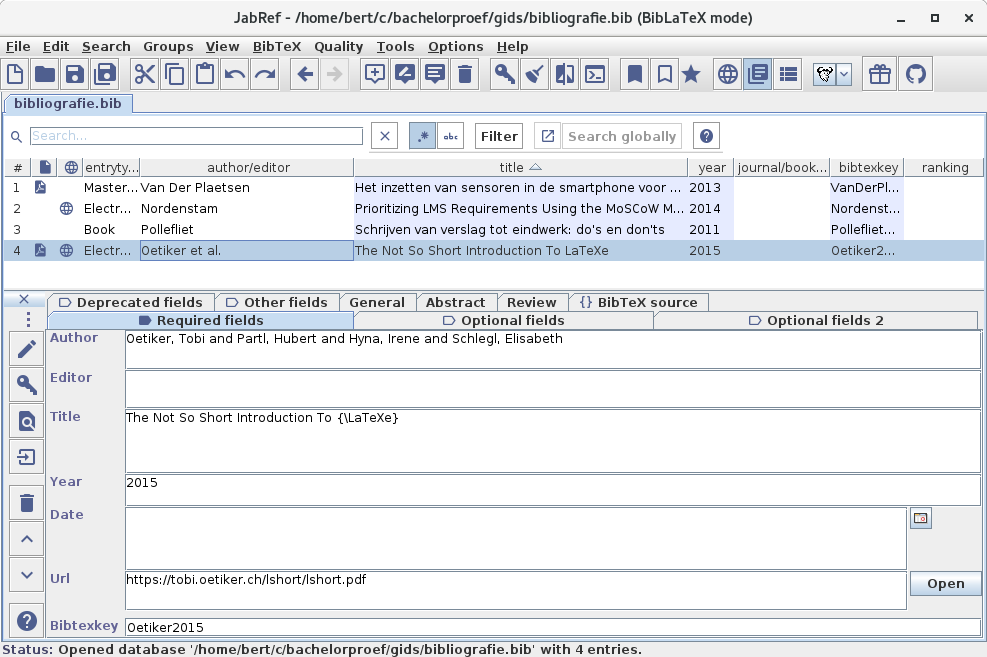
\includegraphics[width=\linewidth]{jabref-screenshot}
  \caption[Jabref]{\textbf{Jabref.} Centraal in de gebruikersinterface vind je een \emph{overzicht} van de verschillende bronnen in deze bibliografische databank, in dit geval vier. De \emph{pdf-icoontjes} links bij de eerste en vierde bron geven aan dat de bron lokaal opgeslagen is als pdf. Als je er op klikt, wordt de pdf geopend. De \emph{wereldbol-icoontjes} bij de tweede en vierde bron duiden op een url die je in de webbrowser kan openen als je er op klikt. Onderaan bevindt zich een \emph{detailvenster} met de bijgehouden gegevens voor de vierde bron. Deze worden opgedeeld in verschillende tabbladen, o.a.~verplichte gegevens (``Required fields''), optionele (``Optional'') en andere (``Other fields''), enz. In dit geval zijn de namen van de auteurs ingevuld (zie Sectie~\ref{sub:algemene_bibliografische_gegevens}). Er zijn in dit geval geen redacteurs (``Editors''), en dat veld is dan ook leeg gebleven. Het veld ``Bibtexkey'' onderaan is automatisch gegenereerd (zie Sectie~\ref{sub:jabref_instellingen}) door te klikken op het \emph{sleutelsymbool} in de knoppenbalk links.}
  \label{fig:jabref}
\end{figure}

\subsection{JabRef instellingen}
\label{sub:jabref_instellingen}

% TODO: richtlijnen bijwerken naar laatste versie Jabref

Je kan Jabref downloaden van \url{http://www.jabref.org/} en installeren op zowel Windows, MacOS als Linux. Bij het voor de eerste keer opstarten is het nuttig om volgende instellingen aan te passen:

\begin{itemize}
  \item Kies in het menu voor File > Switch to BibLaTeX mode. Dit maakt de bestandsindeling van de bibliografische databank compatibel met het aangeboden {\LaTeX}-sjabloon voor de bachelorproef.
  \item Kies in het menu voor Options > Preferences en dan voor de categorie ``BibTeX key generator''. Elke bron in de databank wordt geïdentificeerd door een unieke sleutel die je kan automatisch laten genereren. Je kan de vorm ervan zelf instellen. Het standaardformaat is de familienaam van de eerste auteur gevolgd door het publicatiejaar, bv. ``Knuth1998''. Je kan dit naar eigen smaak aanpassen, maar kies dit vooraf en hou je er aan. Je zal deze sleutel gebruiken om vanuit de tekst te verwijzen naar je bronnen, bv. met het commando \verb|\parencite{Knuth1998}|.
  \item Kies in het Preferences-venster voor de categorie File en geef een directory op voor het bijhouden van PDFs van de gevonden bronnen onder ``Main file directory''. Het is heel interessant om de gevonden artikels te downloaden en onder die directory bij te houden. Nog beter is om als naam van het bestand de BibTeX key te nemen (bv. Knuth1998.pdf). Je kan het bestand dan makkelijk openen vanuit Jabref.
\end{itemize}

Je kan de andere instellingen nakijken en eventueel naar wens aanpassen, maar de hierboven opgesomde zijn de belangrijkste.

\subsection{Algemene bibliografische gegevens}
\label{sub:algemene_bibliografische_gegevens}

De bedoeling van een bibliografie is de lezer toelaten je bronnen zelf op te zoeken en te beoordelen op betrouwbaarheid. Dat betekent dat je voldoende informatie moet opgeven zodat de bron terug te vinden is. Afhankelijk van het soort bron (artikel in een journal, boek, website, enz.) moet je andere informatie opgeven. Dit wordt verderop uitgediept. Drie elementen zijn sowieso \emph{altijd} essentieel: de \textbf{auteur}, de \textbf{titel} van de bron en het \textbf{jaar} (of datum) van publicatie. Als één van deze drie ontbreekt, wordt het bijzonder moeilijk om de oorsprong en de kwaliteit van de bron te evalueren. Dit soort bronnen kan je bijhouden ter info, maar zijn meestal niet geschikt om op te nemen in een bibliografie. Als de auteur onbekend is, is het niet immers mogelijk om te beoordelen of die wel de autoriteit heeft om op een objectieve en diepgaande manier over het onderwerp te schrijven. Als het jaartal niet opgegeven is, is het erg moeilijk om na te gaan in hoeverre deze bron nog niet achterhaald is door recentere ontwikkelingen in het vakgebied.

Enkele tips bij het invullen van auteursnamen:

\begin{itemize}
  \item Noteer de naam van auteurs in de vorm ``Familienaam, Voorna(a)m(en)''. Dus ``Van Vreckem, Bert'' en niet ``Bert Van Vreckem.'' In principe wordt de tweede notatie ook aanvaard, maar dit werkt enkel voor typische angelsaksische namen met een tweede voornaam (bv. ``Donald Ervin Knuth''). De eerste twee woorden worden beschouwd als voornamen, het laatste woord als de familienaam. ``Van'' wordt in dat geval dus verkeerdelijk beschouwd als tweede voornaam.
  \item Als de auteur een bedrijf of organisatie is, met een naam bestaande uit verschillende woorden, zet die dan tussen accolades: bv. ``\{The Linux Foundation\}''. Zoniet probeert {\LaTeX} dit als een persoonsnaam te interpreteren. ``Foundation'' wordt dan de familienaam, ``The'' en ``Linux'' de twee voornamen.
  \item Als je meerdere auteurs hebt, scheid elke naam dan met \texttt{and}, bv. ``Bernard, Anita and Buysse, Jens and Van Vreckem, Bert''.
  \item Na invullen van de auteursna(a)m(en) klik je op de knop met het sleutel-icoon (zie Figuur~\ref{fig:jabref}) om een unieke sleutel te genereren voor deze bron.
  \item Naast een auteurveld is er ook een veld voor eventuele redacteur(en) (\emph{editor}) voorzien. Minstens één van de twee moet ingevuld zijn, soms allebei. Dit gebeurt bijvoorbeeld in een boek dat samengesteld is uit hoofdstukken die telkens door andere auteurs geschreven zijn en waar je naar één bepaald hoofdstuk wil verwijzen. Verderop vind je daar een voorbeeld van.
\end{itemize}

Merk trouwens op dat in een bibliografie \textbf{enkel werken mogen opgenomen zijn waarnaar verwezen wordt vanuit de tekst}. {\LaTeX} doet dit standaard automatisch, dus als je bronnen in de lijst mist, dan betekent dit dat je die niet in de tekst gebruikt hebt.

Probeer telkens zoveel mogelijk informatie bij te houden over je bronnen, zodat het later makkelijker wordt die terug te vinden. Dit is een tijdrovend proces, en niet al deze informatie wordt ook in de bibliografie opgenomen. Het raadplegen van de databank wordt wel een stuk makkelijker. Heb hier voldoende aandacht voor en controleer ook goed het resultaat in de bibliografie zelf. Zijn de auteurs correct weergegeven? Heb je een jaartal? Is er voor een online bron (zie verder) een URL en datum van raadplegen opgegeven? Enz.

Enkele velden die zinvol zijn om altijd trachten in te vullen:

\begin{description}
  \item[Abstract] Samenvatting van het artikel. Dit is meestal de eerste paragraaf van een artikel en wordt altijd duidelijk aangegeven.
  \item[DOI] of ``Digital Object Identifier''. Dit is een unieke code voor artikels in wetenschappelijke publicaties die het opzoeken makkelijker maakt (op voorwaarde dat de DOI gegeven is).
  \item[File] Naam van het bestand met het gedownloade artikel. Je kan vanuit JabRef het artikel openen in een PDF-viewer of desgevallend tekstverwerker.
  \item[Keywords] Kernwoorden die het onderwerp weergeven, gescheiden door komma's.
  \item[Review] Je eigen opmerkingen over deze bron. Waarom heb je deze bijgehouden? Wat is het interessantste dat je er uit geleerd hebt?
  \item[URL] De URL waar je het artikel gevonden hebt. Deze URL wordt niet altijd in de bibliografie opgenomen, maar is altijd nuttig om bij te houden. Je kan vanuit JabRef de website openen in een webbrowser.
  \item[Urldate] de datum waarop je deze bron het laatst hebt geraadpleegd.
\end{description}

\subsection{Specifieke bibliografische gegevens}
\label{sub:specifieke_bibliografische_gegevens}

In deze sectie wordt voor de meest relevante soorten bronnen uitgelegd hoe deze correct bij te houden en in de bibliografie op te nemen. JabRef geeft zelf al enige aanwijzingen over welke informatie minstens nodig is: in het detailvenster (zie Afbeelding~\ref{fig:jabref}) moet je minstens het tabblad ``Required fields'' invullen. Voor elke soort publicatie (zie Sectie~\ref{sub:publicatievormen}) vind je verderop een overzicht van de in te vullen velden en wat die precies betekenen, en hoe de referentie in de literatuurlijst er uit zal zien.

Bij het toevoegen van een nieuwe bron aan een bibliografische databank moet je eerst het type selecteren (zie Afbeelding~\ref{fig:jabref-entrytypes}). Hieronder bespreken we enkel de belangrijkste die relevant zijn voor een bachelorproef.

\begin{figure}
  \centering
  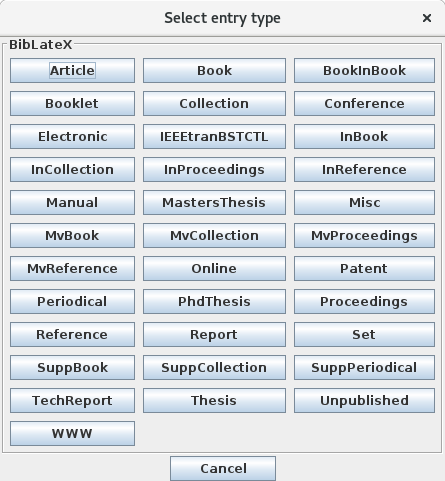
\includegraphics[width=0.6\linewidth]{img/jabref-entrytypes}
  \caption[Soorten bronnen in JabRef]{\textbf{Soorten bronnen in Jabref.} Bij het toevoegen van een nieuwe bron in JabRef (Ctrl+N) moet je eerst het soort publicatie kiezen. Afhankelijk van het soort moet in de literatuurlijst immers andere informatie gegeven worden.}
  \label{fig:jabref-entrytypes}
\end{figure}

\paragraph{Article}

Dit soort bron wordt enkel gebruikt voor artikels die verschenen zijn in een wetenschappelijke journal. Artikels in (vak)tijdschriften of kranten vallen hier \emph{niet} onder. Verplichte velden:

\begin{description}
\item[Author] De naam van de auteur;
\item[Title] De titel van het artikel;
\item[Year] Jaar waarin het artikel verschenen is;
\item[Volume] De jaargang van het tijdschrift waarin het artikel verschenen is;
\item[Number] Het nummer (binnen de jaargang) waarin het artikel verschenen is (soms niet gegeven);
\item[Pages] Paginanummers
\end{description}

Voorbeeld:
\begin{verbatim}
@Article{SabiEtAl2016,
  author       = {Sabi, Humphrey M. and Uzoka, Faith-Michael E. and
                  Langmia, Kehbuma and Njeh, Felix M.},
  title        = {Conceptualizing a model for adoption of cloud
                  computing in education},
  journaltitle = {International Journal of Information Management},
  year         = {2016},
  volume       = {36},
  number       = {2},
  pages        = {183--191},
  doi          = {10.1016/j.ijinfomgt.2015.11.010},
  url          = {http://www.sciencedirect.com/[...]8401215001115},
  abstract     = {Cloud computing is a pervasive computing [...]},
  keywords     = {Cloud computing, Educational technologies, [...]},
  owner        = {bert},
  timestamp    = {2016-09-01},
}
\end{verbatim}

In de bibliografie ziet dit er zo uit: \fullcitebib{SabiEtAl2016}

\paragraph{InProceedings}

Dit soort bron wordt gebruikt voor artikels die gepubliceerd zijn in het verslag (proceedings) van een \emph{wetenschappelijke} conferentie. Verplichte velden:

\begin{description}
  \item[Author] Naam van de auteur(s),
  \item[Title] Titel van het artikel,
  \item[Booktitle] De naam van de conferentie,
  \item[Year] Het jaar waarin de conferentie doorging.
\end{description}

Daarnaast kan je optioneel ook volgende velden invullen:

\begin{description}
  \item[URL] naar de website van de conferentie waar het artikel kan gevonden (eventueel rechtstreeks naar de pdf);
  \item[Urldate] datum waarop je deze bron het laatst geraadpleegd hebt.
  \item[DOI] op voorwaarde dat er één toegewezen is aan dit artikel.
\end{description}

Voorbeeld:
\begin{verbatim}
@InProceedings{VanVreckemEtAl2013,
  author    = {Van Vreckem, Bert and Borodin, Dmitriy and De Bruyn,
               Wim and Now\'{e}, Ann},
  title     = {A Reinforcement Learning Approach to Solving Hybrid
               Flexible Flowline Scheduling Problems},
  booktitle = {Multidisciplinary International Scheduling Conference
               (MISTA) 2013},
  year      = {2013},
  url       = {https://expertise.hogent.be/files/10711623/hffsp_la.pdf},
  urldate   = {2016-09-01},
  abstract  = {In this paper, we present a method based on Learning
               Automata to solve Hybrid Flexible Flowline Scheduling 
               Problems [...].},
  owner     = {bert},
  timestamp = {2016-09-01},
}
\end{verbatim}

In de bibliografie: \fullcitebib{VanVreckemEtAl2013}

\paragraph{InBook}

Dit type gebruik je als je wil verwijzen naar een specifiek hoofdstuk in een boek. Minstens volgende velden moeten dan ingevuld zijn:

\begin{description}
  \item[Author] De auteur(s) van het hoofdstuk,
  \item[Editor] De redacteur(en) van het boek (indien van toepassing),
  \item[Year] Jaartal waarin het boek werd uitgegeven,
  \item[Title] Titel van het \emph{hoofdstuk},
  \item[Pages] Begin- en eindpagina van het hoofdstuk,
  \item[Booktitle] Titel van het \emph{boek},
  \item[Publisher] Naam van de uitgeverij.
\end{description}

Optioneel kan je ook volgende informatie aanvullen:

\begin{description}
  \item[Subtitle of Booksubtitle] ondertitel van het hoofdstuk of boek, resp.,
  \item[Edition] Nummer van de uitgave,
  \item[Location] Stad waar de uitgeverij gevestigd is,
  \item[ISBN] Het ISBN-nummer van het boek (ter info, wordt nooit getoond in de bibliografie).
\end{description}

Bij een boek is het ongebruikelijk om een URL op te geven. Als je bijvoorbeeld ter info voor jezelf de URL van het boek op de website van de uitgever wil bijhouden, doe je dit best in een ander veld, bv. Comment of Review.

Voorbeeld
\begin{verbatim}
@InBook{Meyr2008,
  author       = {Meyr, Herbert},
  title        = {Forecast Methods},
  booktitle    = {Supply Chain Management and Advanced Planning},
  year         = {2008},
  editor       = {Stadtler, Hartmut and Kilger, Christoph},
  booksubtitle = {Concepts, Models, Software, and Case Studies},
  edition      = {4e editie},
  publisher    = {Springer},
  location     = {Heidelberg},
  isbn         = {978-3-540-24814-9},
  pages        = {461--472},
  comment      = {https://www.springer.com/us/book/9783540248149},
  owner        = {bert},
  timestamp    = {2016-09-02},
}
\end{verbatim}


In de bibliografie: \fullcitebib{Meyr2008}

%% TODO: boek, thesis, manual, \ldots

\paragraph{Electronic of Online}

Onder dit type publicatie vallen vrijwel alle online bronnen die niet onder een andere categorie te plaatsen zijn: blogartikels, artikels in online vaktijdschriften of portaalsites, Youtube-video's van presentaties op vakconferenties, online documentatie, enz.

Merk op dat je de algemene website van organisaties, softwarepakketten, enz. \emph{niet} in je literatuurlijst mag opnemen. Deze kan je wel in een voetnoot zetten.

Deze velden moet je verplicht invullen:

\begin{description}
  \item[Author] Auteur(s) van de bron, spreker (in het geval van een video van een lezing op een conferentie), \ldots
  \item[Title] Titel van de bron, lezing, \ldots
  \item[Year] Jaartal van publicatie (of eventueel \textbf{Date}, de dag van publicatie, als die bekend is),
  \item[URL] naar de website waar de bron kan teruggevonden worden,
  \item[Urldate] Datum van laatste raadplegen,
\end{description}

Bij dit soort bronnen worden veel fouten gemaakt bij het refereren. Het is essentieel dat de URL wordt meegegeven en ook de datum van raadplegen. Het web is voortdurend in beweging, en het is mogelijk dat de inhoud van een webpagina in de loop van de tijd verandert (bv. fouten die verbeterd worden) of zelfs dat een website herstructureert en de URL dus op een gegeven manier niet meer geldig is. Door de datum van raadplegen op te geven, bied je de lezer nog de kans om terug te vinden hoe die website er op dat moment in de tijd uitzag, via bijvoorbeeld de Wayback Machine van het Internet Archive\footnote{\url{https://archive.org/web/}}.

Voorbeeld van een blogartikel:

\begin{verbatim}
@Electronic{LewisFowler2014,
  author    = {Lewis, James and Fowler, Martin},
  title     = {Microservices: a definition of this new architectural
               term},
  date      = {2014-03-25},
  url       = {http://martinfowler.com/articles/microservices.html},
  urldate   = {2016-09-01},
  abstract  = {The term "Microservice Architecture" has [...]},
  keywords  = {application architecture, web services, microservices},
  owner     = {bert},
  timestamp = {2016-09-01},
}
\end{verbatim}

In de bibliografie wordt dit: \fullcitebib{LewisFowler2014}

Een ander voorbeeld, deze keer van een presentatie op een vakconferentie die op Youtube is gepubliceerd. Omdat er niet meteen een apart veld voorzien is voor het vermelden van de naam van de conferentie, is die hier in het titelveld verwerkt.

\begin{verbatim}
@Online{Hykes2013,
  author       = {Solomon Hykes},
  title        = {The future of Linux Containers (PyCon 2013)},
  date         = {2013-03-21},
  url          = {https://www.youtube.com/watch?v=wW9CAH9nSLs},
  urldate      = {2016-09-01},
  abstract     = {At PyCon Solomon Hykes shows docker to the
                  public for the first time.},
  owner        = {bert},
  timestamp    = {2016-09-01},
}
\end{verbatim}

In de bibliografie: \fullcitebib{Hykes2013}

\section{Op zoek naar relevante informatie}
\label{sec:op_zoek_naar_relevante_informatie}

Via de HOGENT bib krijg je toegang tot een grote hoeveelheid wetenschappelijke en vakliteratuur die niet publiek beschikbaar zijn. Dit gaat veel verder dan de boeken die in de bib beschikbaar zijn. Daarnaast zijn immers nog elektronische bronnen (ebooks, tijdschriften, enz.) te raadplegen. Ook (goede) bachelorproeven van vorige jaren kan je op deze manier vinden. De catalogus is te raadplegen via \url{https://bib.hogent.be/zoeken/}.

Databanken die niet publiek beschikbaar zijn kan je raadplegen als je op de campus bent, of thuis via Apollox: \url{https://apollox.hogent.be/}. Voor ons vakgebied zijn in het bijzonder volgende databanken interessant:

\begin{itemize}
  \item Elsevier ScienceDirect
  \item Springer Online Journals
  \item Web of Science
  \item Google Scholar
\end{itemize}

Google Scholar is een zoekmachine voor wetenschappelijke literatuur die zowel in publiek toegankelijke (``open access'') als betalende publicaties zoekt. Als je Scholar gebruikt vanop de campus of via Apollox, krijg je automatisch toegang tot de publicaties waar de HOGENT bib een abonnement op heeft.

Andere, publiek toegankelijke startpunten voor het zoeken:

\begin{itemize}
  \item Arxiv.org is een database van Open Acces artikels in een hele reeks onderzoeksdomeinen, o.a. de Computing Research Repository\footnote{\url{http://arxiv.org/corr/home}}.
  
  \item Ook Wikipedia is een goed startpunt voor je onderzoek, maar vergeet niet dat Wikipedia-artikels op zich niet kunnen als referenties. Lees dus de oorspronkelijke bronnen van het artikel na en gebruik die als ze relevant zijn voor je bachelorproef.
  
  \item Er bestaan verschillende portaalsites voor actuele ict-gerelateerde onderwerpen waar technische artikels, presentaties, interviews, enz. op verschijnen, bv. dzone.com\footnote{\url{https://dzone.com/}}, infoq.com\footnote{\url{https://www.infoq.com/}}, enz.
  
  \item Ga op zoek naar voor je vakgebied relevante conferenties, workshops, symposia, enz. Je hoeft je daarbij niet te beperken tot conferenties in eigen land! Voorbeelden zijn Devoxx\footnote{\url{https://devoxx.be/}} (Java), Google IO\footnote{\url{https://events.google.com/io2016/}} (Android), WWDC\footnote{\url{https://developer.apple.com/wwdc/}} (iOS), Configuration Management Camp\footnote{\url{http://cfgmgmtcamp.eu/}} (Linux Systeembeheer), enz. Lanyrd\footnote{\url{http://lanyrd.com/topics/}} is een website waar je vele conferenties kan terugvinden over allerlei onderwerpen en verspreid over heel de wereld.
  
  Meer en meer worden de lezingen van conferenties gefilmd en gepubliceerd op Youtube of Vimeo \footnote{Voor Devoxx bijvoorbeeld op \url{https://www.youtube.com/user/parleysdotcom}}. Je kan ook de sprekers opzoeken en nagaan of ze hun slides gepubliceerd hebben op Slideshare\footnote{\url{https://slideshare.net/}} of Speakerdeck\footnote{\url{https://speakerdeck.com/}}.
  
  \item Zijn er lokaal verenigingen die geïnteresseerd zijn in je vakgebied? Bijvoorbeeld OWASP Belgium\footnote{\url{https://www.owasp.org/index.php/Belgium}} (beveiliging van mobiele en webapplicaties). Je kan naar zulke groepen zoeken via Meetup\footnote{\url{https://meetup.com/}} of ook via LinkedIn\footnote{\url{https://www.linkedin.com/}} (zoek specifiek naar groepen zoals het Belgian IT Infrastructure Network\footnote{\url{https://www.linkedin.com/groups/2092569}}). Kijk eens na of er binnenkort evenementen in de buurt zijn en ga er naartoe.
  
  \item Wie zijn de belangrijkste namen in de ``community''? Keynote-speakers op conferenties, auteurs van de belangrijkste boeken over het onderwerp, enz. Volg deze personen op Twitter, zoek uit of ze een blog hebben, actief zijn op LinkedIn, enz. Lees al wat je kan vinden dat ze geschreven hebben de laatste jaren.
  
  \item Zoek uit of er nieuwsbrieven bestaan over je onderwerp, die periodiek updates uit sturen over de actualiteit binnen dat vakgebied. Voorbeelden zijn Cron.Weekly\footnote{\url{https://www.cronweekly.com/}} (Linux systeembeheer) of DevOps Weekly\footnote{\url{http://www.devopsweekly.com/}}.
\end{itemize}

Het bijhouden van al je bronnen is tijdrovend, maar essentieel voor een goed onderbouwde bachelorproef! Besteed hier dus de nodige aandacht aan en controleer of de informatie over je bronnen correct is ingevuld in JabRef.

Alle relevante informatie die je in de loop van je onderzoek hebt verzameld en gelezen wordt dan gesynthetiseerd in een doorlopende tekst waarin je in je eigen woorden de situatie in het onderzoeksdomein schetst, met op gepaste plaatsen verwijzingen naar de literatuur. Hier gaan we dieper op in in Hoofdstuk~\ref{ch:schrijven}.

\section{Samenvatting}
\label{sec:literatuuronderzoek_samenvatting}

\begin{itemize}
  \item Het doel van de literatuurstudie is om jezelf en de lezer van je bachelorproef voldoende context te geven om het onderwerp ten gronde te begrijpen.
  \item Er zijn drie soorten bronnen: primaire (resultaten van eigen onderzoek), secundaire (publicaties in wetenschappelijke of vakliteratuur) en tertiaire (encyclopedieën en zoekindexen).
  \item In een bibliografie horen enkel \emph{secundaire} bronnen thuis.
  \item Zet je bibliografische databank op (bv. met Jabref) voordat je op zoek gaat naar informatie over je onderwerp en hou van wat je vindt nauwgezet zoveel mogelijk informatie bij.
  \item Zorg dat je altijd minstens de auteur, titel en jaartal hebt en daarnaast minstens alle andere verplichte informatie voor dat type publicatie correct noteert.
  \item Naast het raadplegen van publiek toegankelijke bronnen is het ook interessant om via de HOGENT bib informatie over je onderwerp op te zoeken.
  \item Gebruik de APA stijl.
\end{itemize}


